\documentclass[a4paper,12pt]{article}

\usepackage{Packages}
\usepackage{subfigure}
\usepackage{amsmath}


\begin{document}
\begin{titlepage}

\begin{center}

% Upper part of the page. The '~' is needed because \\
% only works if a paragraph has started.

\includegraphics[width=0.6\textwidth]{./Figures/TUe}~\\[2cm]


%\vspace*{10cm}

% Title
\HRule \\[0.4cm]
{ \huge \bfseries 2IMM20 - Foundations of datamining\\[0.3cm] }
\HRule \\[1.5cm]
\textbf{Assignment 2}


% Author and supervisor

\vfill

\begin{table}[h]
\begin{tabular}{ll}
\textbf{Students:} & \\
Joris van der Heijden & (0937329)\\
Bram van der Pol & (0780042)\\

\\
\textbf{Email addresseses:} & \\
j.j.m.v.d.heijden@student.tue.nl \\
a.f.v.d.pol@student.tue.nl \\
\\
\textbf{Supervisors:} &\\
Dr.ir. Joaquin Vanschoren
\\

%\textbf{Supervisors:} & \\
%Dr. M.Holenderski \\
\end{tabular}
\end{table}



% Bottom of the page
\large
{ Eindhoven, \today}

\end{center}


\end{titlepage}
 %included in part 1

\tableofcontents %included in part 1

\section*{Nepalese character recognition}
\subsection*{1}
{\it Evaluate k-Nearest Neighbors, Logistic Regression and RandomForests with their default
settings.
\begin{itemize}
\item{Take a stratified 10\% subsample of the data.}
\item{Use the default train-test split and predictive accuracy. Is predictive accuracy a good scoring measure for this problem?}
\item{Try to build the same models on increasingly large samples of the dataset (e.g. 10\%,
20\%,...). Plot the training time and the predictive performance for each. Stop when the
training time becomes prohibitively large (this will be different for different models).}
\end{itemize}
The pyhton code is shown in appendix \ref{AQ21}.

\begin{figure}[H]
\hfill
\makebox[\textwidth][c]{{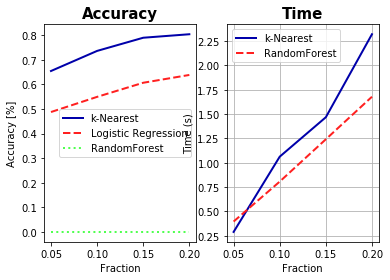
\includegraphics[width=12cm]{./Figures/output_15_1}}}
\hfill
\caption{Predictive accuracy as a function of the subsample data.}
\label{Q21image}
\end{figure}

Figure \ref{Q21image} shows that the accuracy of the k-Nearest and Logistic regression algorithm does not show a clear trend. This can be due to used randomness of the train and test samples. The predictive accuracy is due to this not a good measure for this problem. 

\subsection*{2}
{\it Optimize the value for the number of neighbors $k$ (keep $k < 50$) and the number of trees
(keep $n_{estimators} < 100$) on the stratified 10\% subsample. Use 10-fold crossvalidation and plot $k$ and $n_{estimators}$ against the predictive accuracy. Which value of $k, n_{estimators}$ should you pick?}
Because the simulation took too long for the 10\% subsample only 1\% is taken as the subsample. 
\begin{figure}[H]
\hfill
\makebox[\textwidth][c]{
\subfigure[]{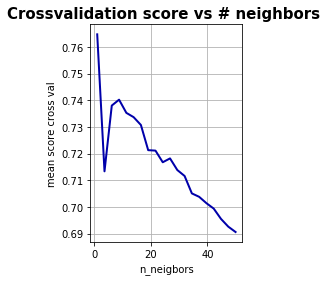
\includegraphics[width=6cm]{./Figures/output_17_1}}
\subfigure[]{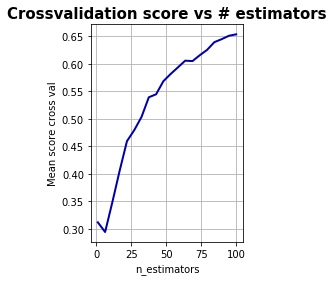
\includegraphics[width=6cm]{./Figures/output_17_3}}}
\hfill
\caption{}
\label{Q22}
\end{figure}
As can been seen in figure \ref{Q22} is that the number of neigbors should be set to 1 and the number of trees to 100. 

\subsection*{3}
{\it For the RandomForest, optimize both $n_{estimators}$ and $max_{features}$ at the same time on the entire dataset. - Use a nested cross-validation and a random search over the possible values, and measure the accuracy. Explore how fine-grained this grid/random search can be, given your computational resources. What is the optimal performance you find? - Hint: choose a nested cross-validation that is feasible. Don’t use too many folds in the outer loop. - Repeat the grid search and visualize the results as a plot (heatmap) $n_{estimators}\cdot max_{features} \rightarrow ACC$ with ACC visualized as the color of the data point. Try to make the grid as fine as possible. Interpret the results. Can you explain your observations? What did you learn about tuning RandomForests?}
\begin{figure}[H]
\hfill
\makebox[\textwidth][c]{{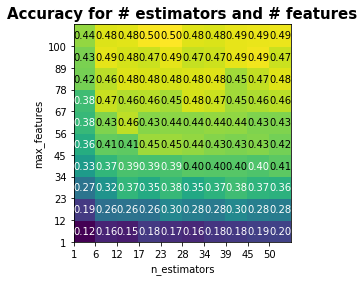
\includegraphics[width=12cm]{./Figures/output_19_1}}}
\hfill
\caption{Accuracy for the random forest for different maximum features and number of estimators numbers. This is done for 1\% of the total data set (due to the lack of computer power and time).}
\label{•}
\end{figure}
The percentage has a big influence for the accuracy prediction. The 

\section*{4}
\subsection*{1}
{\it Do a bias-variance analysis of both algorithms. For each, vary the number of trees on a log scale from 1 to 1024, and plot the bias error (squared), variance, and total error (in one plot per algorithm). Interpret the results. Which error is highest for small ensembles, and which reduced most by each algorithm as you use a larger ensemble? When are both algorithms under- or over-fitting? Provide a detailed explanation of why random forests and gradient boosting behave this way. - See lecture 3 for an example on how to do the bias-variance decomposition - To save time, you can use a 10\% stratified subsample in your initial experiments, but show the plots for the full dataset in your report. In [ ]: from sklearn.model}

\begin{figure}[H]
\hfill
\makebox[\textwidth][c]{{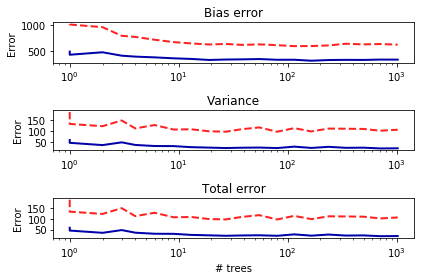
\includegraphics[width=12cm]{./Figures/output_24_1}}}
\hfill
\caption{•}
\label{•}
\end{figure}
\section{Appendix}
\subsection{Code question 2.1}
\label{AQ21}


\subsection{Code question 2.2}



\end{document}
